\chapter{O Computador Visível: Uma base para a computação desplugada?} 

A proposta prática da disciplina será a de desenvolver materiais didáticos para a realização de uma experiência com computação desplugada voltada ao ensino de fundamentos da ciência da computação para comunidades indígenas.

Antes de entrarmos no que representa esse desafio em relação à comunidade, este capítulo lhe apresentará os princípios de um simulador de computador chamado Computador Visível, desenvolvido em 2004 pelo Prof. Jorge Fernandes.

Vamos entender o que é o computador visível, e verificar se ele pode ser base para uma experiência rica em desenvolvimento de material didático, considerando a proposta da computação desplugada.

\begin{figure}
    \centering
    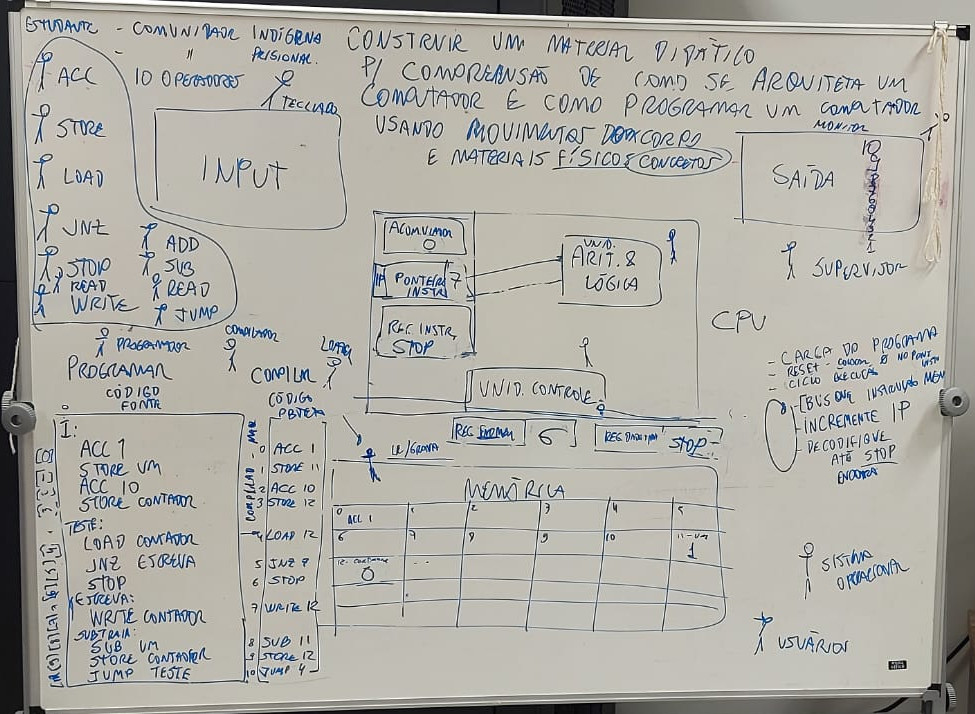
\includegraphics[width=1\textwidth]{2-ComputadorVisivel/imgs/vc0-conversa-livia.jpeg}
    \caption{Esquema geral de funcionamento de um computador digital, por Jorge Fernandes.}
    \label{fig:vc0}
\end{figure}

